\chapter{The predictor/corrector integration scheme}

\begin{figure}[]
  \centering
  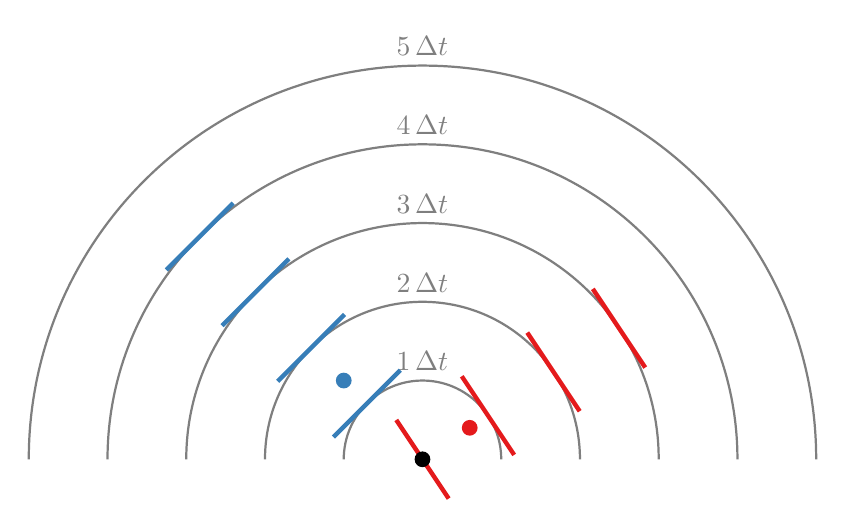
\begin{tikzpicture}[>=latex, scale=1.0]

  \definecolor{Set1-3-1}{RGB}{228,26,28}
  \definecolor{Set1-3-2}{RGB}{55,126,184}

  \foreach \i in {1,2,3,4,5} {
    \draw[thick, opacity=0.5] (\i, 0) arc (0:180:\i);
    \node[above, opacity=0.5] at (0, \i) {$\i \, \Delta t$};
  }

  \fill[color=Set1-3-1] (0.6, 0.4) circle (0.1);
  \begin{scope}[rotate=33.6901]
    \foreach \i in {0,1,2,3} {
      \draw[ultra thick, Set1-3-1] (\i,-0.6) -- (\i, 0.6);
    }
  \end{scope}


  \fill[Set1-3-2] (-1, 1) circle (0.1);
  \begin{scope}[rotate=135]
    \foreach \i in {1,2,3,4} {
      \draw[ultra thick, Set1-3-2] (\i,-0.6) -- (\i, 0.6);
    }
  \end{scope}

  \fill[black] (0, 0) circle (0.1);

  \end{tikzpicture}
  \caption{\label{fig:retardation problem} Illustration of the ``retardation problem'' in solving coupled delay differential equations.
    The filled points show particle locations and the colored tangent lines indicate historical quantities of $\vb{P}$  used in the interpolation scheme developed in \cref{ch:quantum dots}. 
    Because $\abs{\vb{r}_{\bullet \textcolor[RGB]{228,26,28}{\bullet}}} < c \, \Delta t$, determining $\qty{\vb{E}(\bullet, t),\vb{P}(\textcolor[RGB]{228,26,28}{\bullet}, t)}$ requires knowledge of $\qty{\vb{P}(\textcolor[RGB]{228,26,28}{\bullet}, t), \vb{E}(\bullet, t)}$.
  }
\end{figure}

\section{Motivation}

In principle, any standard numerical ODE integrator will work just fine for integrating \cref{eq:liouville,eq:rotating liouville} for a single quantum system.
In practice, however, the retarded coupling between systems introduced by \cref{eq:integral operator,eq:radiated envelope} makes this decidedly more complicated.
These retardation effects turn the 
These equations will have nonintegral retardation factors (i.e.\ $\Delta r/(c \, \Delta t) \not \in \mathbb{Z}$) for any geometry except a linear chain, thus to determine the unknown function ``between'' timesteps we turn to the polynomial interpolation scheme formulated in \cref{ch:quantum dots}.
Given the complexity of tabulating interpolation coefficients and their dependence on $\Delta t$, this automatically excludes variable-step integrators as well as integrators that require an intermediate (mid) step (such as RK4). 

\section{Determination of $\mathcal{P}_w^{(0, 1)}$, $\mathcal{C}_w^{(0, 1)}$}

\begin{figure}
  \centering
  \begin{subfigure}{0.4\textwidth}
    \centering
    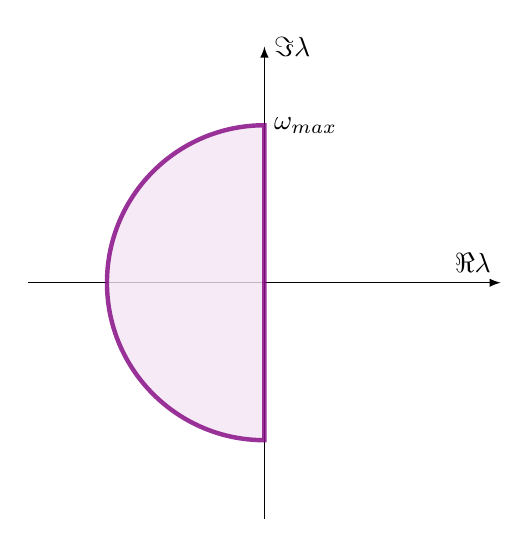
\begin{tikzpicture}[>=latex]
      \draw[->] (0,-3) -- (0, 3) node[right] {$\Im \lambda$};
      \draw[->] (-3,0) -- (3, 0) node[anchor=south east] {$\Re \lambda$};

      \draw[ultra thick, violet, fill=violet!10, opacity=0.8] (0,2) arc(-90:90:-2) -- (0,2) -- cycle;
      \node[right] at (0, 2) {$\omega_\text{max}$};
    \end{tikzpicture}
    \caption{\label{fig:filled semidisk}}
  \end{subfigure}
  \hspace{1cm}
  \begin{subfigure}{0.4\textwidth}
    \centering
    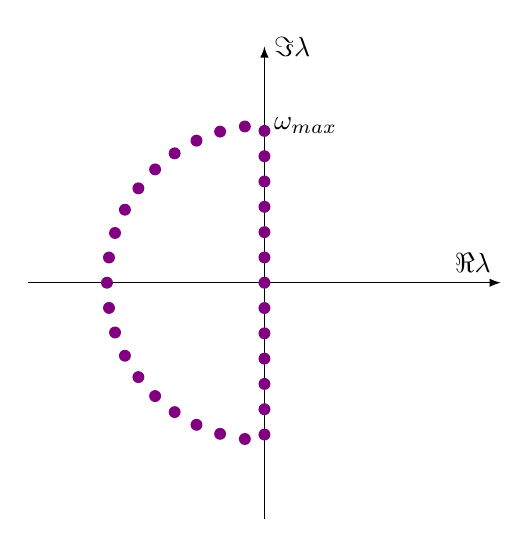
\begin{tikzpicture}[>=latex]
      \draw[->] (0,-3) -- (0, 3) node[right] {$\Im \lambda$};
      \draw[->] (-3,0) -- (3, 0) node[anchor=south east] {$\Re \lambda$};

      \foreach \point in {{0.,0.},{0.,0.32135},{0.,0.642699},{0.,0.964049},{0.,1.2854},{0.,1.60675},{0.,1.9281},{-0.248801,1.98446},{-0.563079,1.9191},{-0.862852,1.8043},{-1.1404,1.64301},{-1.38856,1.43941},{-1.60096,1.19872},{-1.77212,0.927148},{-1.89762,0.631695},{-1.97424,0.319969},{-2.,1.22465*10^-16},{-1.97424,-0.319969},{-1.89762,-0.631695},{-1.77212,-0.927148},{-1.60096,-1.19872},{-1.38856,-1.43941},{-1.1404,-1.64301},{-0.862852,-1.8043},{-0.563079,-1.9191},{-0.248801,-1.98446},{0.,-1.9281},{0.,-1.60675},{0.,-1.2854},{0.,-0.964049},{0.,-0.642699},{0.,-0.32135}}
      {
        \fill[violet] (\point) circle (0.5ex);
      }
      \node[right] at (0, 2) {$\omega_\text{max}$};
    \end{tikzpicture}
    \caption{\label{fig:discrete semidisk}}
  \end{subfigure}
  \caption{\label{fig:semidisk} Selection of the $\lambda_n$ parameters used in determining the predictor/corrector coefficients.
  }
\end{figure}

Let $x(t)$ denote the solution to a given ordinary differential equation.
Assuming $x(t)$ contains little power above some threshold angular frequency $\omega_\text{max}$, we may approximate $x(t)$ with a collection complex-valued exponentials such that
\begin{equation}
  x(t) \approx \sum_{\ell = 0}^{N_\lambda - 1} w_\ell e^{\lambda_\ell t}
  \label{eq:exponential approximation}
\end{equation}
for a given set of complex-valued $\lambda_\ell$ arguments (explained below) and $w_\ell$ weights (never calculated explicitly).

If $x(t)$ and $\partial_t x(t)$ have known values at equidistant points $t_0, t_1, \ldots, t_{W - 1}$ on the interval $\qty[-1, 1]$ (thus $\Delta t = 2/(W - 1)$), the prediction step of \cref{eq:predictor} requires
\begin{equation}
  x(t_W) = \sum_{j = 0}^{W - 1} p_j x(t_j) + p_{j + W} \, \partial_t x(t_j).
\end{equation}
Inserting \cref{eq:exponential approximation} gives
\begin{equation}
  A \vb{p} = \vb{b}
  \label{eq:predictor vector}
\end{equation}
where
\begin{subequations}
\begin{align}
  A_{ij} &= \begin{cases}
    e^{\lambda_i t_j}, & 0 \leqslant i < N_\lambda; \; 0 \leqslant j < W \\
    \lambda_i e^{\lambda i t_{j - W}}, & 0 \leqslant i < N_\lambda; \; W \leqslant j < 2 W
  \end{cases} \\
  b_i &= e^{\lambda_i t_W}.
\end{align}
\end{subequations}
Accordingly, we use a minimum-norm least-squares procedure to determine the predictor coefficients $\vb{p}$ in \cref{eq:predictor vector}.
An identical technique follows for determining the corrector coefficients.
As the corrector step \cref{eq:corrector} stipulates
\begin{equation}
  x(t_W) = \qty(\sum_{j = 0}^{W - 1} c_j x(t_j) + c_{W + j} \, \partial_t x(t_j)) + c_{2W} \, \partial_t x(t_W)
\end{equation}
(with $\partial_t x(t_W)$ having come from evaluating the particular ODE at time $t_W$), the linear system for $\vb{c}$ becomes
\begin{equation}
  \tilde{A} \vb{c} = \vb{b}.
\end{equation}
Here,
\begin{equation}
  \tilde{A}_{ij} = \begin{cases}
    A_{ij}, & 0 \leqslant i < N_\lambda; \; 0 \leqslant j < 2W \\
    \lambda_i e^{\lambda_i t_W}, & 0 \leqslant i < N_\lambda; \; j = 2W
  \end{cases}
\end{equation}
$\vb{b}$ remains unchanged, and the same least-squares procedure determines $\vb{c}$.

Having derived the predictor/corrector coefficients for $h = 2/(W - 1)$ (i.e.\ a uniform spacing between $W$ timepoints on the interval $\qty[-1, 1]$), the coefficients determined above require only a slight modification to accommodate systems with any $\Delta t$.
Noting that the formulation thusfar remains invariant under time translation and that the substitution $\tau = \alpha t$ (equivalently $\alpha = \Delta t/h$) turns
\begin{subequations}
\begin{equation}
  \pdv{\varphi(t)}{t} = \lambda \varphi(t)
\end{equation}
into
\begin{equation}
  \pdv{\varphi(\tau)}{\tau} = \frac{\lambda}{\alpha} \varphi(\tau),
\end{equation}
\end{subequations}
we need only scale the coefficients multiplying $\partial_t x(t_j)$ by $\alpha$ to adjust for other step sizes.

\section{Determination of the $\lambda_i$}

where the $\lambda_\ell$ lie within the complex left-semidisk $S_{\omega_\text{max}} = \qty{\lambda \in \mathbb{C} \, | \Re{\lambda} \leqslant 0, \abs{\lambda} \leqslant \omega_\text{max}}$ (\cref{fig:filled semidisk}).
Rather than choosing $\lambda_\ell$ from throughout $S_\rho$, the maximum modulus principle ensures that arguments taken from the boundary of $S_\rho$ in \cref{fig:discrete semidisk} will incur the maximum approximation error in \cref{eq:exponential approximation}. 
As a result, an approximation using these boundary $\lambda_\ell$ accurately recovers the behavior of all modes with arguments in $S_\rho$.



